\documentclass[10pt]{extarticle}

% ---------- Packages ----------
\usepackage{fancyhdr}
\usepackage{geometry}
\usepackage{hyperref}
\usepackage{xcolor}
\usepackage{amsmath, amsfonts, bm}
\usepackage{subcaption}
\usepackage{graphicx}
\graphicspath{{images/}}
\usepackage{tikz}
\usepackage{nomencl}
\usepackage{array}
\usepackage{pdflscape}
\usepackage{multicol}
\usepackage[export]{adjustbox}
\usepackage[utf8]{inputenc}
\usepackage{parskip}
\usepackage{ifthen}
\usepackage[section]{placeins} % floats never cross into the next section

\usetikzlibrary{shapes.geometric}
\usetikzlibrary{arrows.meta, arrows}

% ---------- Page setup ----------
\geometry{
    a4paper,
    total={170mm,257mm},
    left=20mm,
    top=20mm
}

% ---------- Headers and footers ----------
\pagestyle{fancy}
\pagenumbering{arabic}

\fancyhead[L]{Dossier de définition - Iphigénie 60}
\fancyfoot[C]{}
\fancyfoot[R]{\thepage}

% ---------- Hyperlinks ----------
\hypersetup{
    colorlinks=true,
    linkcolor={blue!50!black},
    citecolor={blue!50!black},
    urlcolor={blue!80!black}
}

% ---------- Nomenclature ----------
\makenomenclature
\setlength{\nomlabelwidth}{3.2cm}
\renewcommand{\nomgroup}[1]{%
  \ifthenelse{\equal{#1}{A}}{\item[\textbf{Geometry}]}{%
  \ifthenelse{\equal{#1}{B}}{\item[\textbf{Kinematics}]}{%
  \ifthenelse{\equal{#1}{C}}{\item[\textbf{Statics}]}{}}}}

% ---------- Float placement ----------
% let LaTeX place figures/tables (here, top, bottom, own page) and allow more of them per page
\renewcommand{\topfraction}{0.85}
\renewcommand{\bottomfraction}{0.7}
\renewcommand{\textfraction}{0.15}
\renewcommand{\floatpagefraction}{0.6}
\setcounter{topnumber}{3}
\setcounter{bottomnumber}{2}
\setcounter{totalnumber}{4}

% ---------- Equation numbering ----------
\numberwithin{equation}{subsection}

% ---------- Custom commands ----------
\newcommand{\todo}[1]{%
    \textcolor{red}{TODO: #1}%
}

\begin{document}

\begin{titlepage} % Suppresses headers and footers on the title page

	\centering % Centre everything on the title page

	\scshape % Use small caps for all text on the title page

	\vspace*{\baselineskip} % White space at the top of the page

	%------------------------------------------------
	%	Title
	%------------------------------------------------

	\rule{\textwidth}{1.6pt}\vspace*{-\baselineskip}\vspace*{2pt} % Thick horizontal rule
	\rule{\textwidth}{0.4pt} % Thin horizontal rule

    \vspace{0.75\baselineskip} % Whitespace above the title

	{\LARGE \hfill \\ Dossier de définition \\ Iphigénie 60 \\ \hfill \\} % Title

	\vspace{0.75\baselineskip} % Whitespace below the title

	\rule{\textwidth}{0.4pt}\vspace*{-\baselineskip}\vspace{3.2pt} % Thin horizontal rule
	\rule{\textwidth}{1.6pt} % Thick horizontal rule

	\vspace{2\baselineskip} % Whitespace after the title block

	%------------------------------------------------
	%	Team
	%------------------------------------------------

	{\large Team Leaders}

	\vspace{0.25\baselineskip}

	{\scshape\Large Yaroslav Knyazkov \\ Paul Retourné \\ Issam Kerrouche \\ Marija Krsteska \\ Antonio Makhlouf \\ \hfill \\} % Team leaders

	\vspace{0.75\baselineskip}

	{\large Team Members}

	\vspace{0.25\baselineskip}

	\begin{multicols}{3}
	\small\centering
	Andrey Fourcade \\ Brian Lee \\ Sangram Choudhury \\ Marlow Squire \\ Tanakrit Penganunsart \\ Joel Xaviar Peiris \\ Fernando Martins \\ Khadija Hajiyeva \\ Jekaterina Elizabete Barala \\ Oliver Bizzi \\ Alex Chaland \\ Tymofii Bulba \\ Yves Zhang \\ Chibuba Okoye \\ Yahya Abdulmalek \\ Mikhail Ilin \\ Julie Cavadini \\ Jules Garidou \\ Antoine Francés \\ Gaelle Abi Ghanem \\ Shafinaz Shahrin Manita \\ Arthur Lelièvre \\ Radovan Stefancin \\ Louis Garidou \\ Antoine Ligneul \\ Maya Su Mutlu \\ Julie Barnes \\ Syed Ghazi Ali Abidi
	\end{multicols}

	\vfill % Whitespace between team list and publisher logo

	%------------------------------------------------
	%	Publisher
	%------------------------------------------------

    2026 % Publication year

	{\large CLES-FACIL} % Publisher

    \vspace{0.3\baselineskip} % Whitespace under the publisher logo

    \begin{figure}[h]
        \centering
        
\includegraphics[width=0.35\linewidth]{logo-cles-facil.png}
    \end{figure}
\end{titlepage}


\newpage

\tableofcontents

\newpage

% ---------- Nomenclature entries ----------
% \nomenclature[A00]{$symbol$}{description}
% \printnomenclature

\newpage

% ---------- TODO: sections ----------
\section{Goals \& Experiments}
\subsection{Goals}
The design of the rocket is based on the goals set during its definition. The goals are in order :
\begin{enumerate}
	\item Launch the rocket --- we have not launched a rocket in the past two years, so this is our main priority.
	\item Get interesting results from our two experiments --- see more details in the experiment section.
	\item Cement the club knowledge and create a solid team for the following years.
	\item Optimize the rocket --- using the knowledge of new members, we aim to optimize the rocket both aerodynamically and structurally, using CFD, FEA, and parametric and topology optimization.
	\item Optimize and predict the rocket's trajectory --- using an in-house simulator, we want to predict the trajectory as accurately as possible (verified against StabTraj) and stabilize the pitching and rolling dynamics using theoretical models, not only experimental ones (e.g.\ diameter-based static margin).
	\item Get live feedback from the experiments and the rocket state during the flight.
\end{enumerate}

\subsection{Experiments}
The following paragraphs describe the main experiments planned for the Iphigénie 60 rocket.

\paragraph{Air brake} is the main experiment. The current design status and controller approach are detailed in section \ref{sec:sys-airbrake}.
\begin{itemize}
    \item \textit{Goal:} characterize and validate the air brake's ability to control the rocket's drag so that it reaches a target apogee $h_{\textrm{target}}$, given that the motor's thrust is sized to overshoot $h_{\textrm{target}}$ by default.
    \item \textit{Parameters to study:} additional drag force (or drag coefficient) produced by the air brake as a function of deployment angle, the resulting apogee, and the vertical velocity/acceleration profile during the braking phase.
    \item \textit{Measurement range and precision:} \todo{}
    \item \textit{Hypothesis:} without the air brake, the motor drives the rocket to overshoot $h_{\textrm{target}}$; by extending drag flaps during ascent, the air brake can bleed off the excess energy and bring the achieved apogee down to $h_{\textrm{target}}$.
    \item \textit{Expected outcome:} the achieved apogee lands within a few percent of $h_{\textrm{target}}$, markedly closer than the uncontrolled (brakeless) apogee predicted in table \ref{tab:1}.
\end{itemize}

\paragraph{Reaction wheel} experiment. Background on our previous attempts is given in section \ref{sec:sys-reaction-wheel}.
\begin{itemize}
    \item \textit{Goal:} analyze whether a motor-driven reaction wheel can control the rocket's roll rate in flight, counteracting roll induced by fin misalignment and roll--pitch coupling.
    \item \textit{Parameters to study:} roll rate over time, reaction-wheel motor torque/current, and the coupling between roll rate and pitch rate.
    \item \textit{Measurement range and precision:} \todo{}
    \item \textit{Hypothesis:} a motor-driven reaction wheel can actively damp the rocket's roll rate independently of fin-induced torque, keeping it near zero during the camera-recording phase of flight despite roll--pitch coupling.
    \item \textit{Expected outcome:} the roll rate measured with the reaction wheel active is substantially lower than in our previous (uncontrolled) attempts, giving steadier camera footage.
\end{itemize}

\subsection{Additional elements}

\paragraph{Telemetry}

The onboard sensors will transmit live data to a ground station, the goal is to be able to follow the exact state of the rocket live during the flight and record the data in addition to the onboard storage.\\
We will also include cameras to record the flight and we might try to have a live video feed from the rocket.

\paragraph{Radar tracking station}

We are collaborating with a previous member of the club that is currently building a radar tracking station.\\
A turret carrying the antenna is pointed at the rocket tracking everything that is possible about it, this will then allow us to compare measurements with the onboard sensors.\\
This project is developped independently from the FUSEX and does not require any modification except a small reflector that will be placed in the nosecone thus if it is not finished in time or cannot be used during C'Space it will not affect the FUSEX.
We have more details available if needed.

\subsection{Timeline}
The project is planned according to the following milestones:
\begin{itemize}
    \item Design finished --- end of December.
    \item Optimizations finished --- mid-January.
    \item Manufacturing finished --- end of February.
\end{itemize}
 \newpage
\section{Mechanical}
\subsection{Initial design}
Configuration 

Motors

\subsection{Systems}
\subsubsection{Air frame}
\subsubsection{Air brake}
The air brake team is currently in the design stage.
Based on reports from other projects, we have selected and adapted one of the existing air-brake extension mechanisms, shown in figure \ref{fig:airbrake-mechanism}.

The team is organized into eight parts: design (CAD), drivetrain mechanics (motor and gear sizing), air-brake mechanics (aerodynamic and friction force evaluation), structural, aerodynamics (CFD), opening-controller design, and trajectory-controller design.

\begin{figure}[ht]
    %\includegraphics{}
    \caption{Selected air-brake extension mechanism.}
    \label{fig:airbrake-mechanism}
\end{figure}

\todo{specify design constraint --- "current design is within the \_\_\_"}
\subsubsection{Structural}

\subsection{Tests}
FEA + structural

CFD \newpage
\section{Electrical} \newpage
\section{Team structure}
\subsection{About}
Our team is mainly composed of INSA Lyon students, with the exception of students from
\begin{itemize}
    \item INSA Strasbourg
    \item \todo{Julie} IUT Lyon 1
    \item \todo{Oliver}.
\end{itemize}
The teams operate in English, due to the significant number of international members.

\subsection{Organization}
Our club's main leaders are Paul Retourné (FX27 lead), Yaroslav Knyazkov (Mechanical lead), and Issam Kerrouche (Electrical lead).

The Fusex project is split into an electrical team and a mechanical team, with the mechanical team further subdivided into systems.
Each team is run by a team lead, and team meetings are held weekly.
Tasks are tracked in a shared spreadsheet and divided by team, as shown in figure \ref{fig:team-structure}.
We are in the process of developing a spreadsheet for variable management and an inquiry system, where one team can request a parameter from another team.

\begin{figure}[ht]
    \centering
    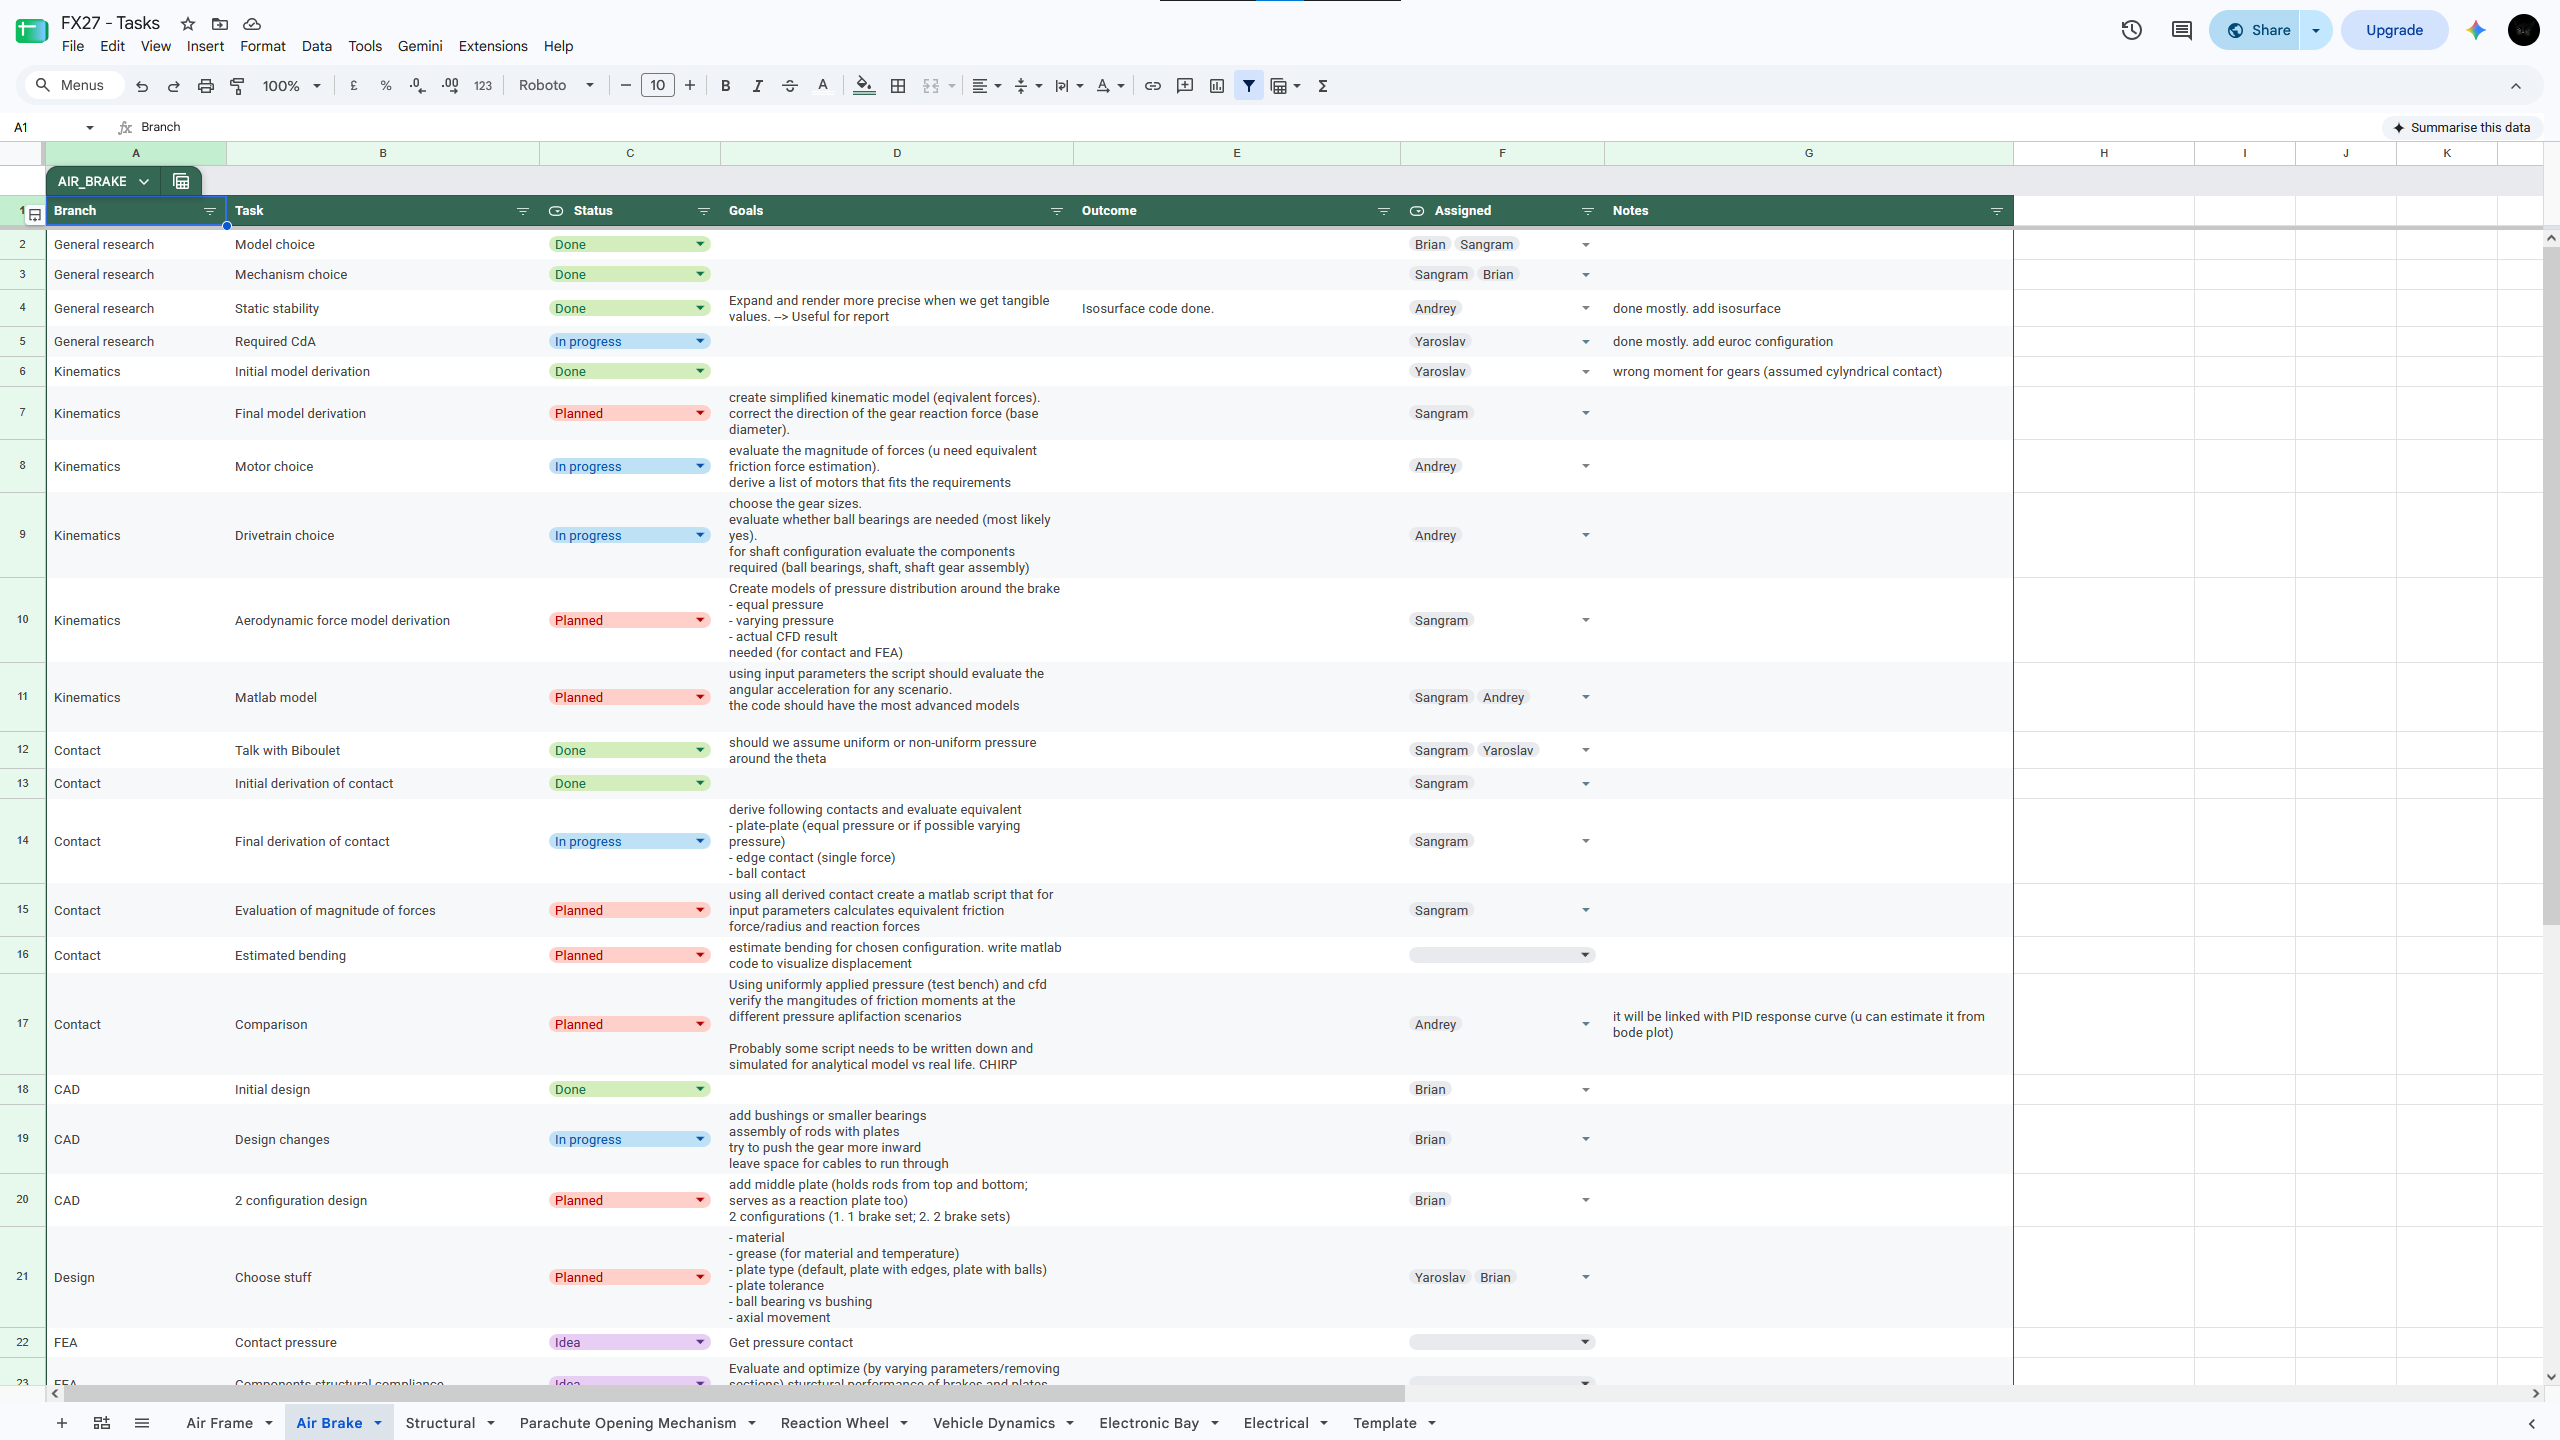
\includegraphics[width=\textwidth]{Tasks.png}
    \caption{Team structure and task breakdown.}
    \label{fig:team-structure}
\end{figure} \newpage
% No questions
% \section{Questions}
\begin{enumerate}
    \item Notre conception actuelle utilise un cône arrière (\textit{tail cone}) composé de deux parties : (1) un cône arrière Pro54 du fabricant, et (2) une surface supplémentaire placée dessus afin qu'il soit au ras du tube de la fusée. Nous comprenons que les cônes arrière ne sont pas fournis par le C'Space. Nous en achèterons un pour une autre compétition, mais nous aimerions savoir si nous pouvons utiliser cette conception au C'Space, ou si elle n'est pas autorisée.

    \item Nous croyons nous souvenir qu'au C'Space, il est interdit de larguer quoi que ce soit depuis la fusée (sauf si l'élément reste attaché), pour des raisons de sécurité et de protection de l'environnement. Cette année, nous prévoyons de développer un bouton de rail qui se détache pendant le lancement. Cela serait-il acceptable ? Notre conception s'inspire de cette vidéo : \url{https://youtu.be/LnunMEopsb8?t=83}

    \item If we are allocated the Pro75 motor, would we be able to switch to the Pro54 if a design change comes up later? This is unlikely, but we would like to know just in case.

    \item What are the rail dimensions? We have only been able to find the maximum rocket dimensions, not the rail size, which would be useful for the rocket's vehicle dynamics.

    \item Regarding the 3000\,m apogee limit, we understand it is a maximum. Should we aim slightly lower, e.g.\ within 100\,m of the 3000\,m limit? Or is it acceptable as long as StabTraj predicts less than 3000\,m?

    \item If we fly transonic, would it be acceptable to still use composite fins provided we demonstrate their strength? We are in contact with another team using the same method we intend to use; their predicted maximum loading is 35\,kg per fin, which should be sufficient.
\end{enumerate}

\end{document}
